\newpage
\subsection{Расчет предварительной стоимости продукции}
\label{bp:calculation}

Расчет предварительной стоимости продукции производится в системе 1С: УПП. 

Менеджер собирает всю информацию от клиента по новому изделию. 
Менеджер получает требования от клиента, уточняет размеры, условия доставки, марки. Требования обычно приходят устно, через мессенджеры, по электронной почте.
Менеджер в системе 1С: УПП производит предварительный расчет стоимости продукции двумя способами:
\begin{enumerate}
    \item Создает документ ''Расчет стоимости продукции'' (рис. \ref{pic:I.2.4..jpg}) на основании предварительно сформированного им черновика ТК (рис. \ref{pic:II.4.jpg}) и с использованием кнопки ''Расчет стоимости'' и ''Расчет Маржи'' производит расчет.
    \item Не формируя ТК создает документ ''Расчет стоимости продукции'', заполняет все необходимые характеристики. Далее производит расчет с использованием кнопок ''Расчет стоимости'' и ''Расчет Маржи''.
\end{enumerate}

В некоторых случаях менеджер может завысить расчетную стоимость изделия. 

Результаты расчетов согласовываются с коммерческим отделом ООО ТД ''ФОРМАТ'' и только после согласования оформляется Коммерческое предложение (рис. \ref{pic:I.4.jpg}).
Заказчик ответным письмом высылает менеджеру согласованное предложение, указывает свои реквизиты 
% (рис. \ref{pic:I.2.1.jpg}) 
для заключения договора. 
% Менеджер при необходимости может запросить дополнительную информацию (рис. \ref{pic:I.2.2.jpg}), необходимую для заключения договора.

Весь внутренний документооборот фиксируется в программе ''Первая Форма'' (рис. \ref{pic:I.5.2..jpg}).
Учет договоров с контрагентами осуществляется в системе 1С: УПП.
После согласования проекта договора через программу ''Первая Форма'' менеджер должен создать заявку на заведение нового контрагента (рис. \ref{pic:I.5.2.jpg}) в системе 1С: УПП.
Нового контрагента в систему 1С: УПП заводит Бухгалтерия.

Оригиналы подписанных договоров хранятся в бухгалтерии.






%Менеджер выполняет расчет предварительной цены продажи в таблице MS Excel (рис. \ref{pic:dd5}), подбирает параметры. Цена указывается за м2 по марке картона. Четкого алгоритма расчета цены продажи не выявлено.


%Цены по стоимости за марку картона зафиксированы за 2 месяца в таблице MS Excel  (рис. \ref{pic:dd3}). Коммерческий директор выполняет расчет цены в форме файл \ref{pic:dd3} и выкладывает цены в сетевой доступ для менеджеров. Менеджер добавляет в цену расчет на упаковку, доставку и получает цену продажи.
%Менеджер формирует КП (рис. \ref{pic:dd4}). Шаблона четкого нет. 

%Менеджер высылает коммерческое предложение клиенту.  Заказчик в ответ высылает менеджеру согласованное предложение с реквизитами для заключения договора. 
%Менеджер формирует договор поставки и высылает заказчику на согласование.

%После согласования коммерческого предложения Менеджер 
%создает вручную проект договора (рис. \ref{pic:dd5}), создает карточку договора в системе СБИС.

%Номер договора присваивает юрист по запросу менеджера. Менеджер в системе СБИС создает спецификацию по клиенту, заводит в справочник Номенклатура в СБИС новую позицию, указывает размеры, площадь, тип гофры, цвет картона, размеры упаковки .
%Система СБИС присваивает номенклатурный номер.
%Менеджер заполняет спецификацию в СБИС (рис. \ref{pic:dd6_1}). Менеджер в СБИС ставит в обработку (фиксирует), печатает спецификацию в СБИС (рис. \ref{pic:dd6_1}). Менеджер создает бланк договора и спецификацию в системе СБИС. 
%Менеджер создает счет в СБИС. Номенклатура выбирается по созданной спецификации. 
%Менеджер печатает счет на оплату (рис. \ref{pic:dd8}).

%Менеджер отправляет клиенту договор с приложением в виде спецификации, счет на предоплату при необходимости.
%Клиент подписывает договор, спецификацию и оплачивает счет.



%После согласования цены Менеджер должен начать разработку ТК (см. процесс ''Подготовка производства'' \ref{bp:Prepare}).




% \begin{figure}
% \begin{center}
% 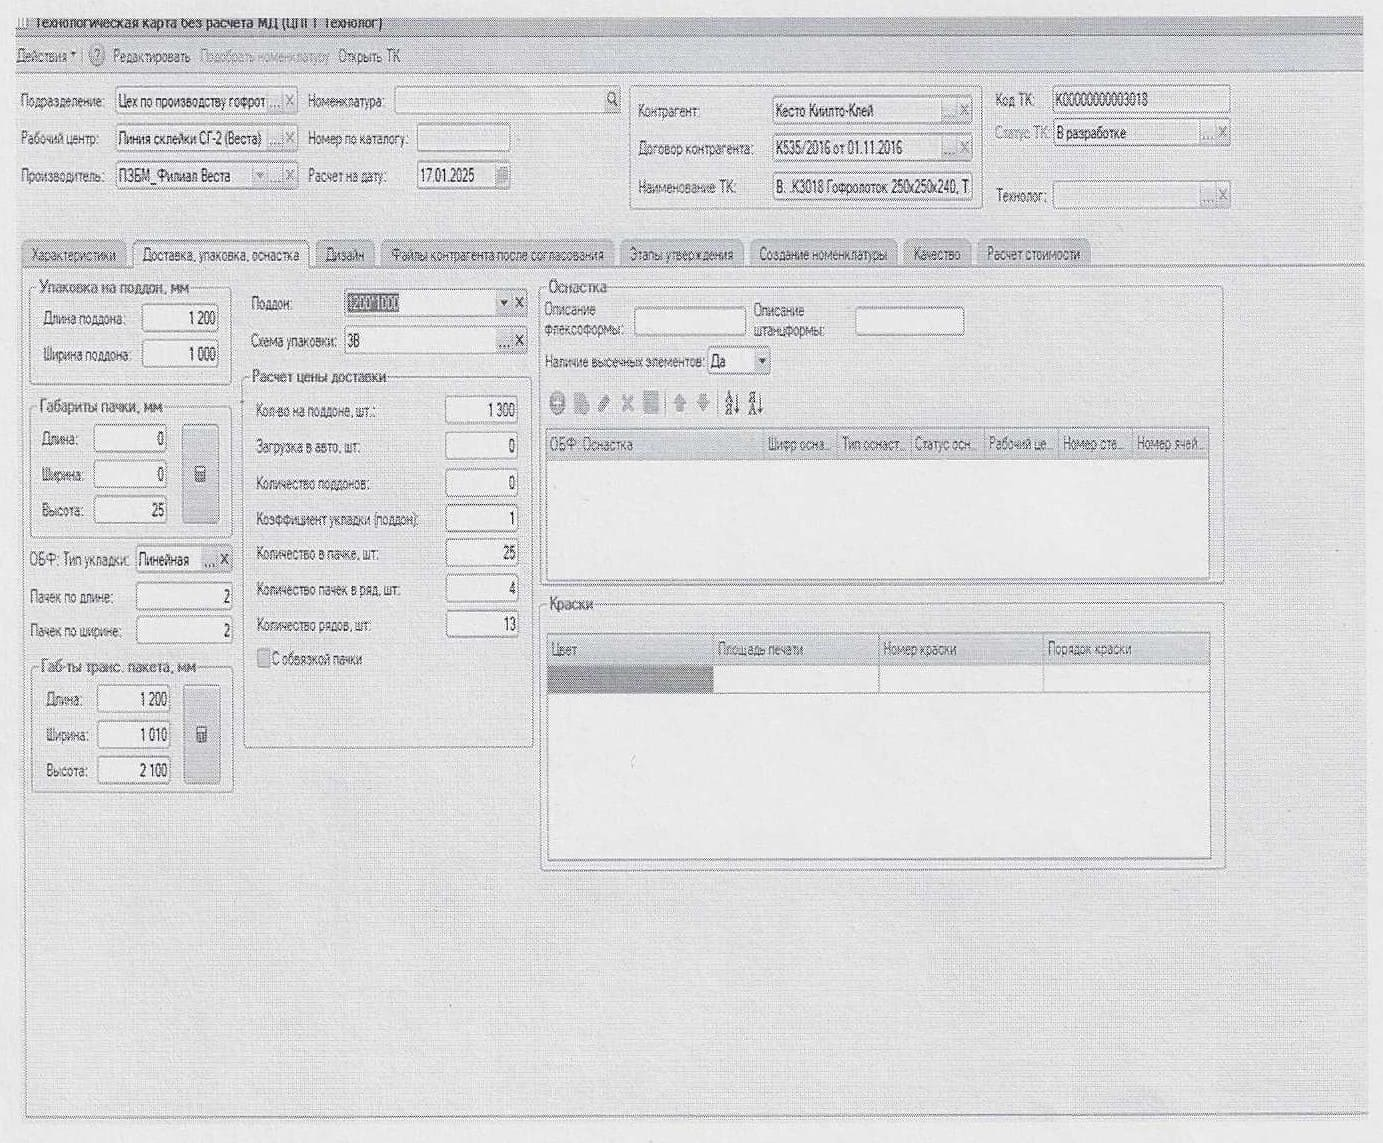
\includegraphics[height=0.5\textheight, width=1.3\textwidth, keepaspectratio]{Pics/II.4.jpg}
% \end{center}
% \caption{Форма Технологическая карта}
% \label{pic:II.4.jpg}
% \end{figure}
% \clearpage

\begin{figure}
\begin{center}
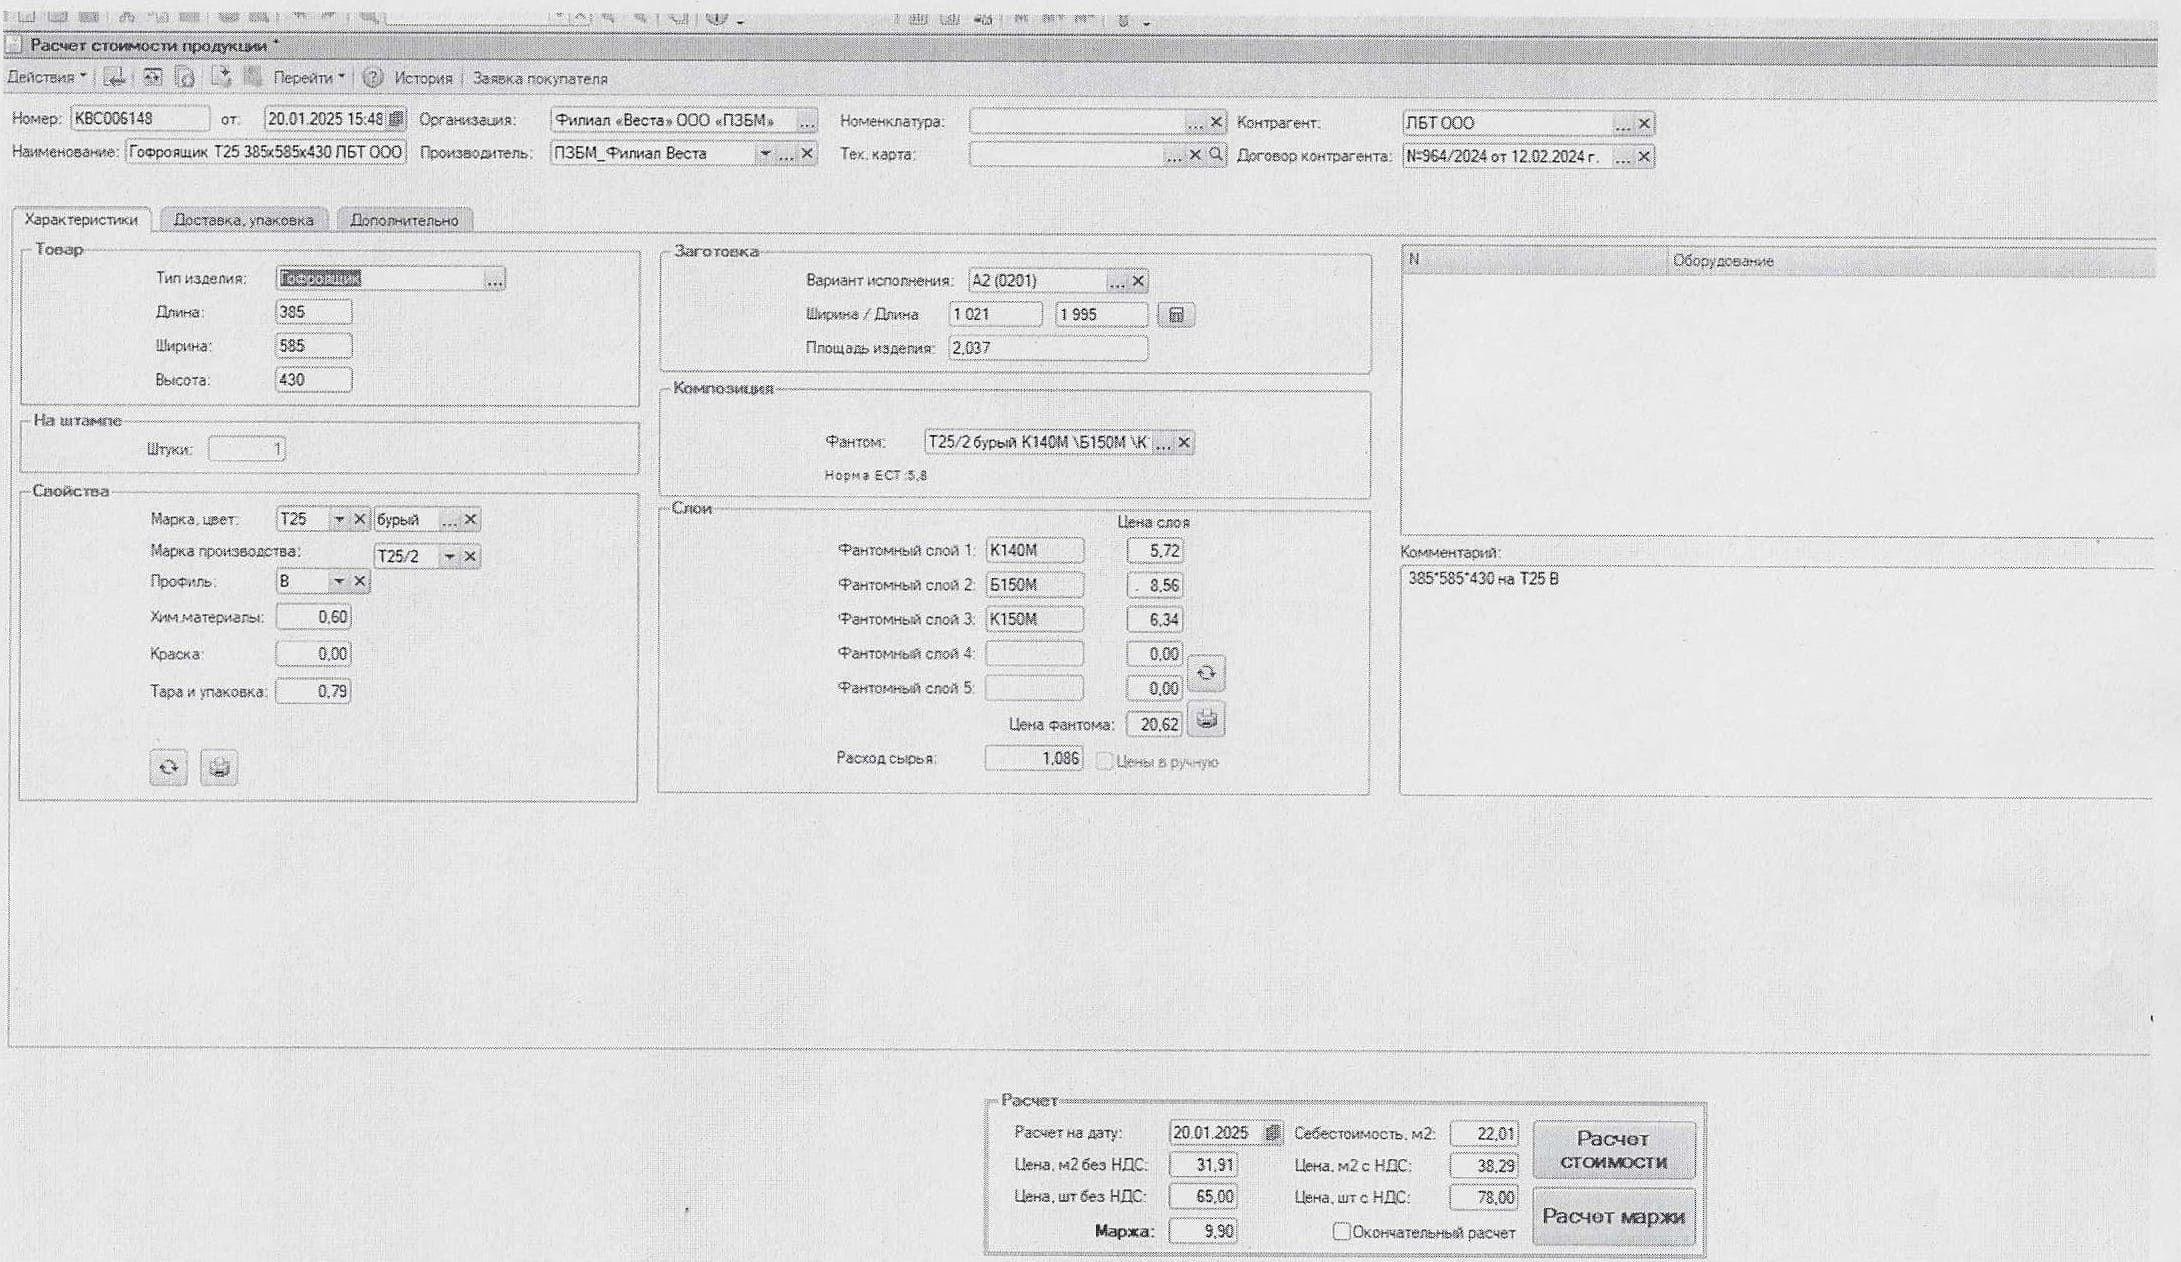
\includegraphics[height=0.38\textheight, width=1.3\textwidth, keepaspectratio]{Pics/I.2.4..jpg}
\end{center}
\caption{Расчет стоимости продукции}
\label{pic:I.2.4..jpg}
\end{figure}
\clearpage

\begin{figure}
\begin{center}
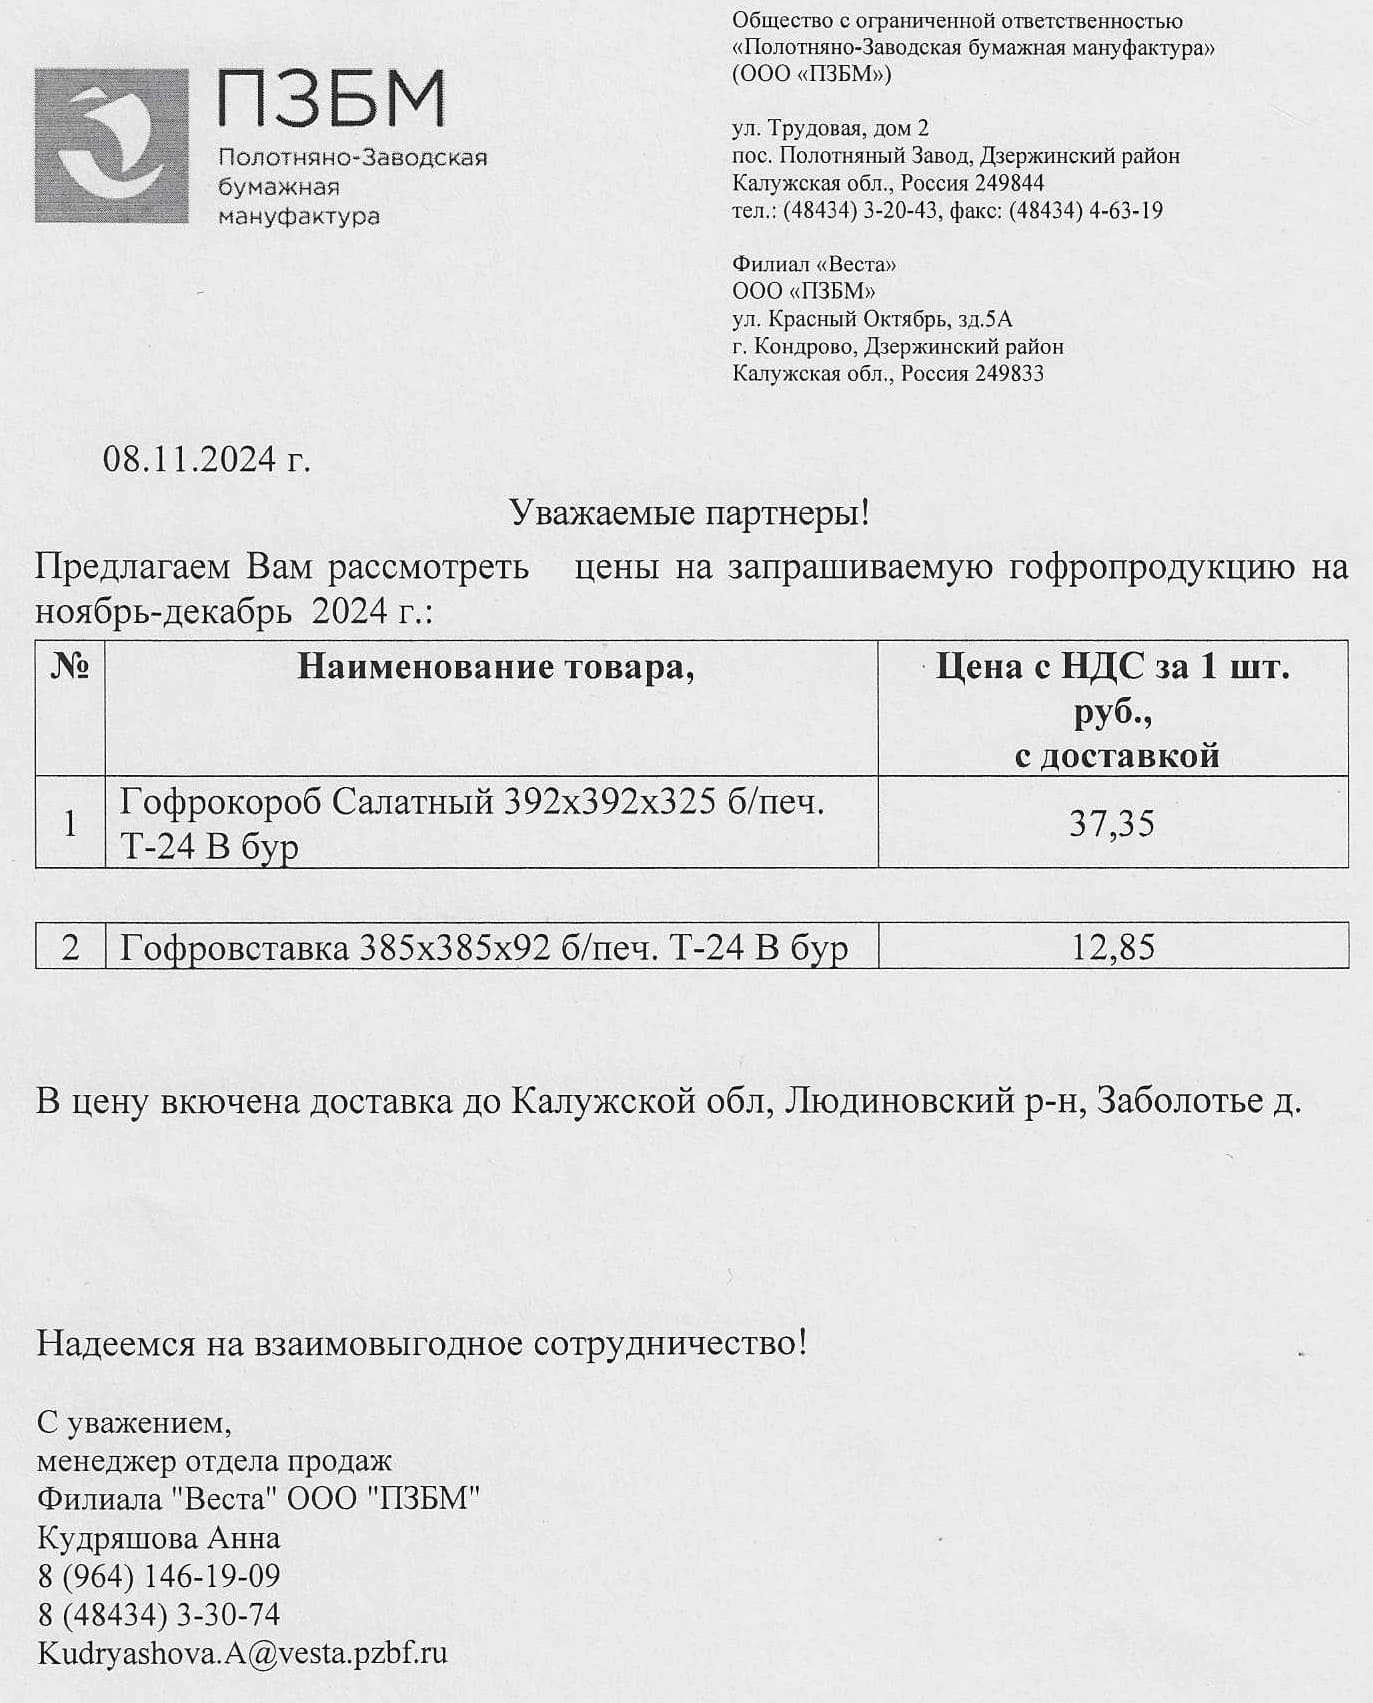
\includegraphics[height=0.8\textheight, width=1.5\textwidth, keepaspectratio]{Pics/I.4.jpg}
\end{center}
\caption{Пример Коммерческого предложения}
\label{pic:I.4.jpg}
\end{figure}
\clearpage

% \begin{figure}
% \begin{center}
% 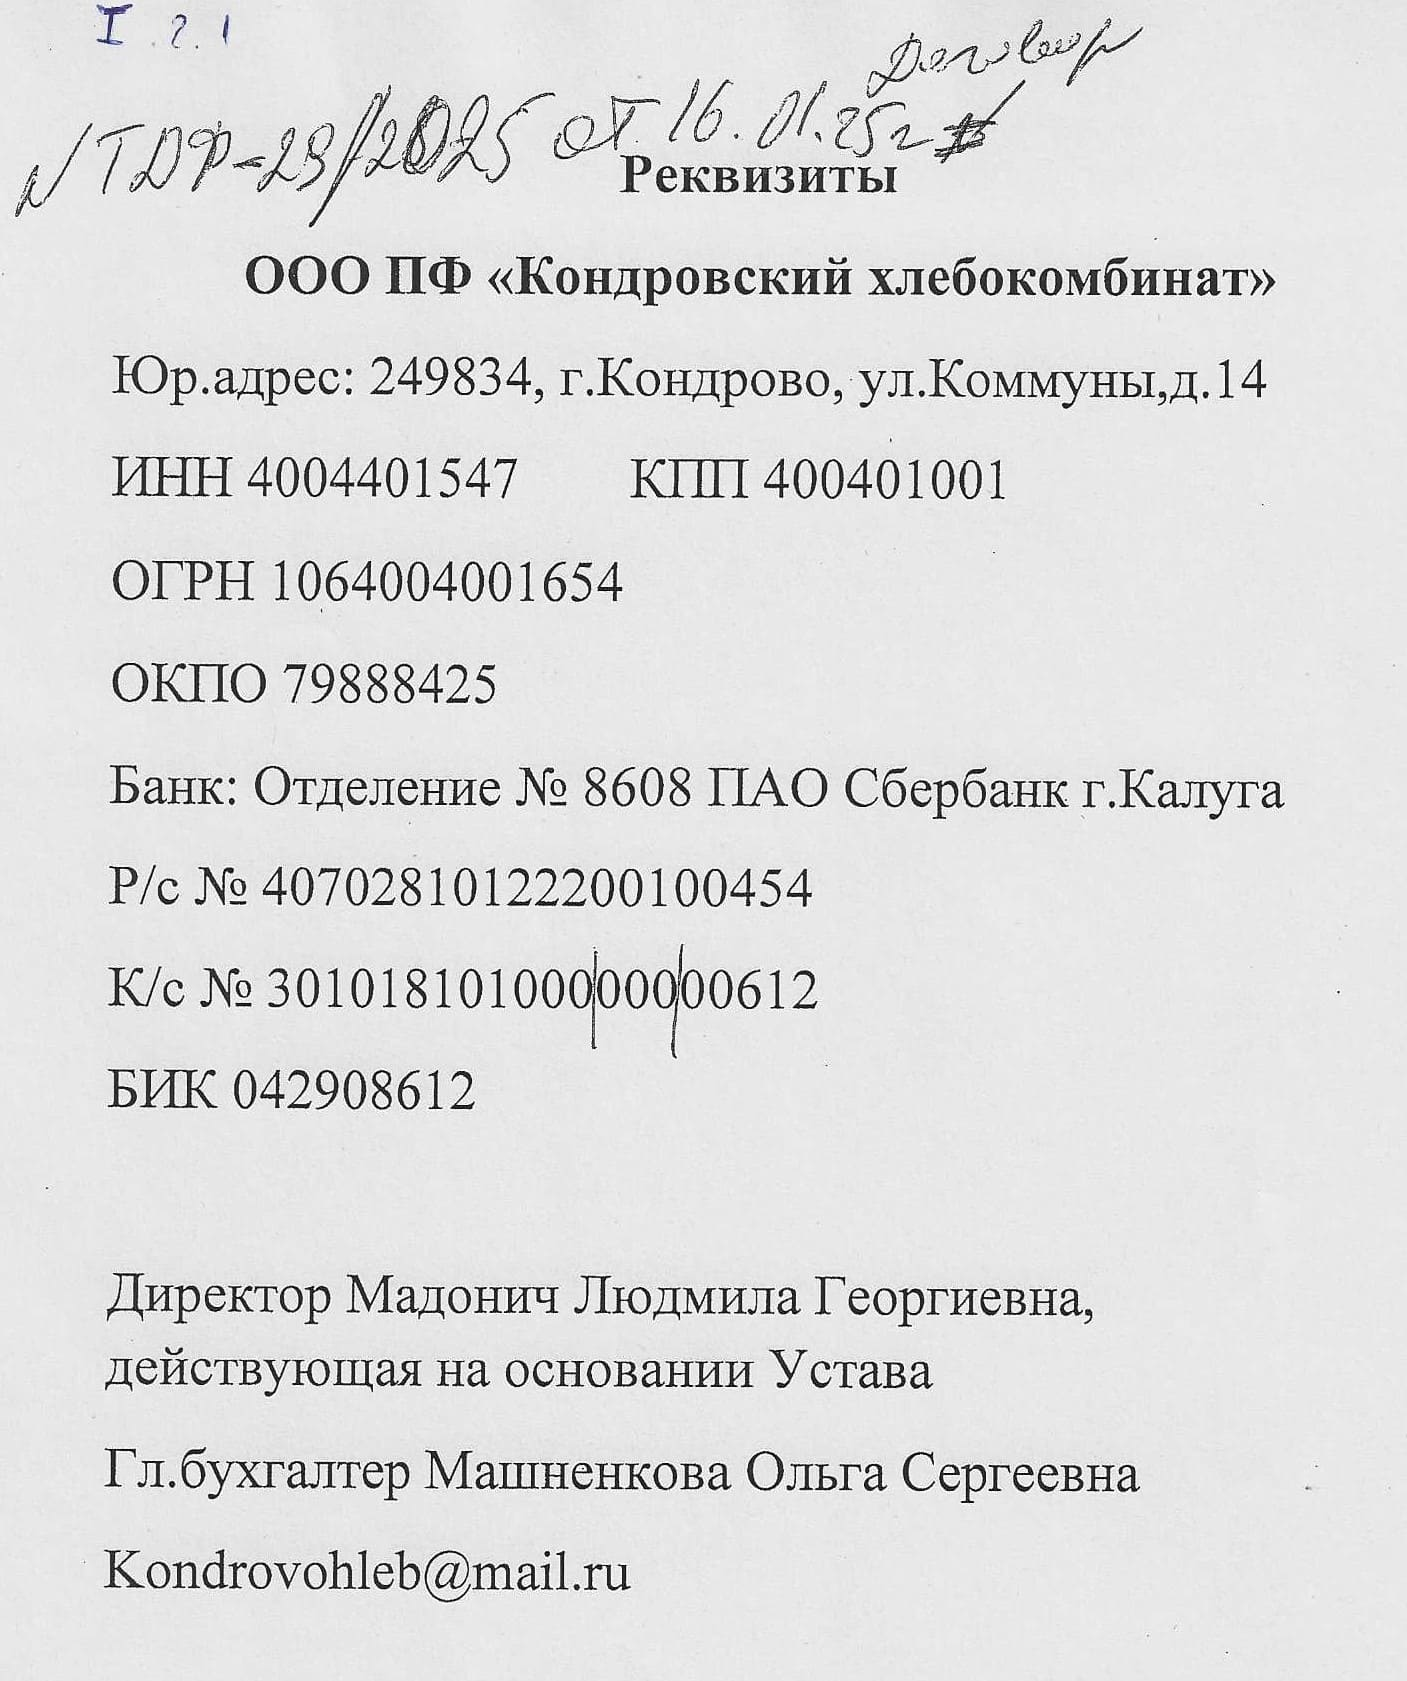
\includegraphics[height=0.6\textheight, width=1.5\textwidth, keepaspectratio]{Pics/I.2.1.jpg}
% \end{center}
% \caption{Пример реквизитов заказчика}
% \label{pic:I.2.1.jpg}
% \end{figure}
% \clearpage

% \begin{figure}
% \begin{center}
% 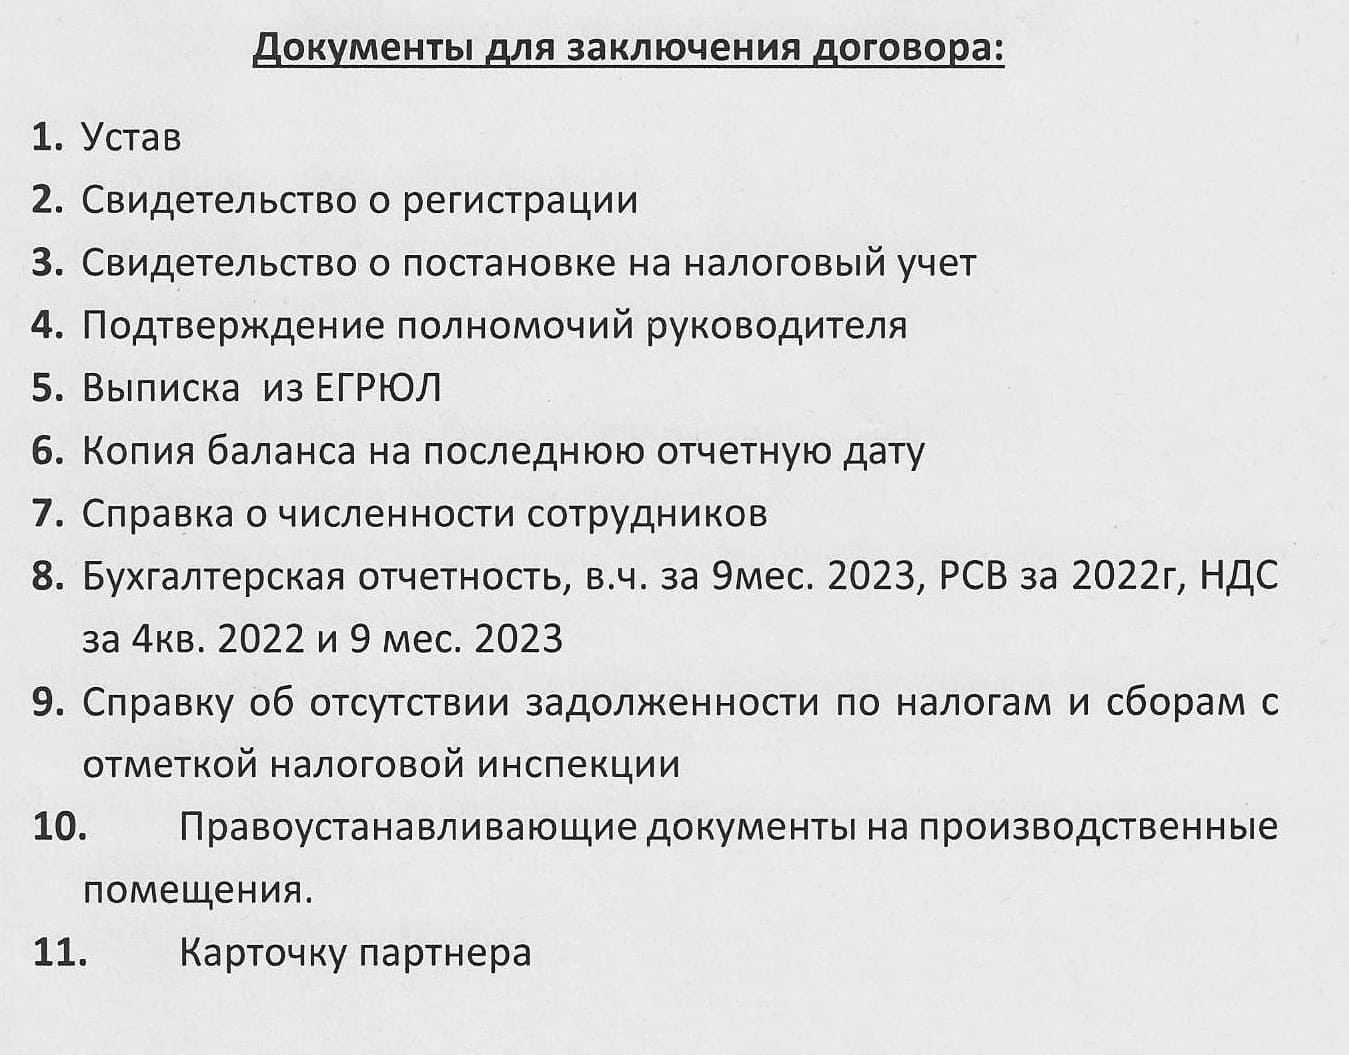
\includegraphics[height=0.45\textheight, width=1.5\textwidth, keepaspectratio]{Pics/I.2.2.jpg}
% \end{center}
% \caption{Требуемые документы для заключения договора}
% \label{pic:I.2.2.jpg}
% \end{figure}
% \clearpage


\begin{figure}
\begin{center}
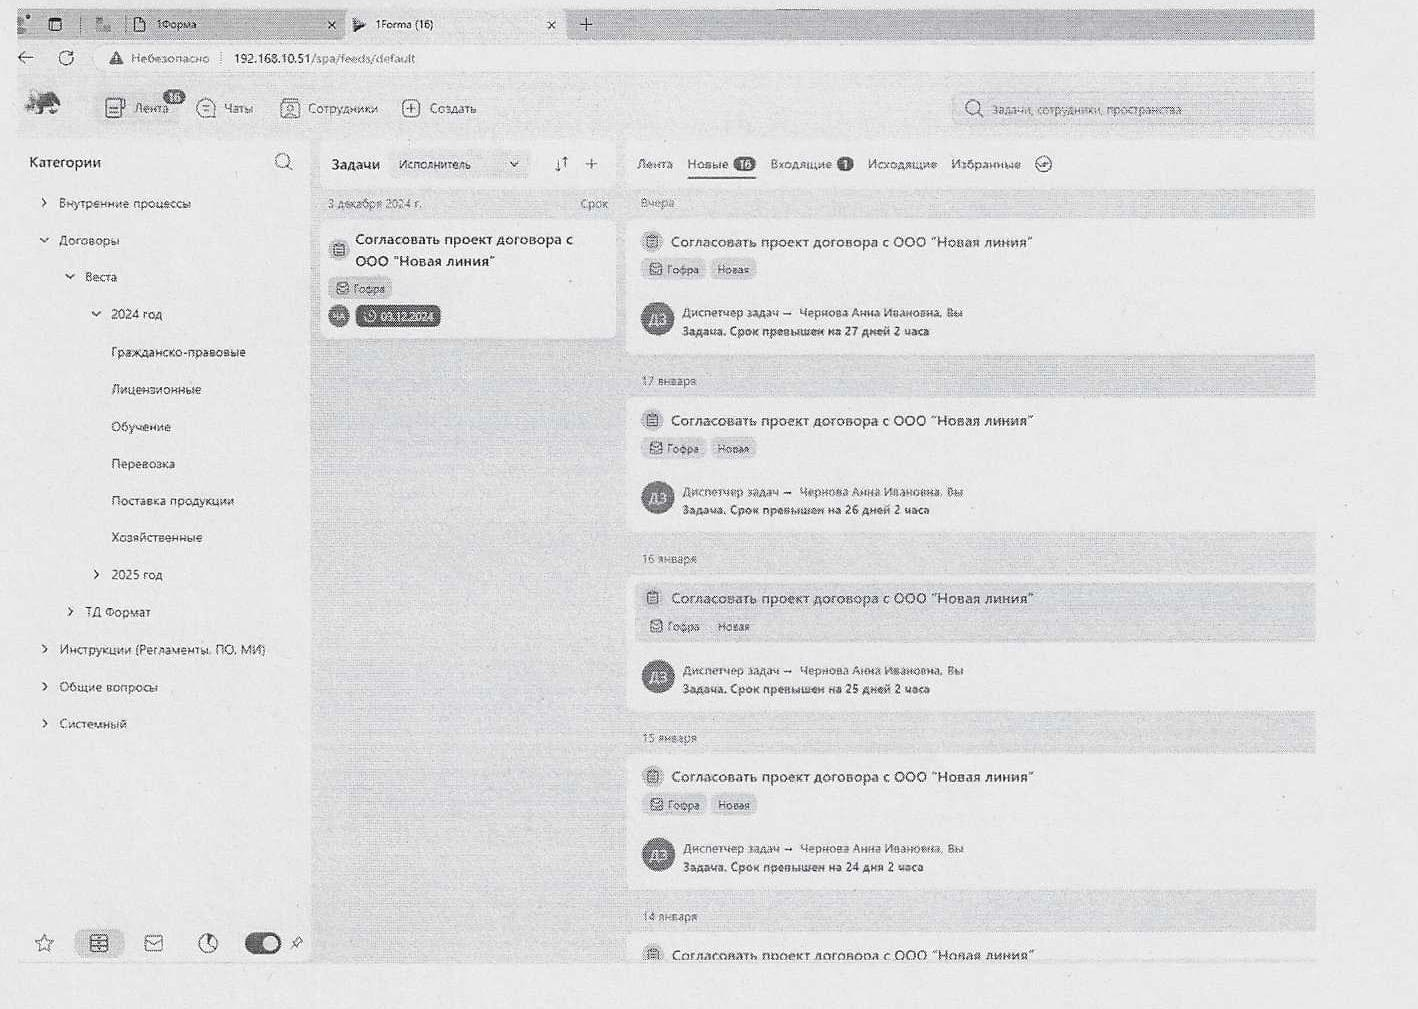
\includegraphics[height=0.45\textheight, width=1.5\textwidth, keepaspectratio]{Pics/I.5.2..jpg}
\end{center}
\caption{Программа ''Первая форма''}
\label{pic:I.5.2..jpg}
\end{figure}
\clearpage

\begin{figure}
\begin{center}
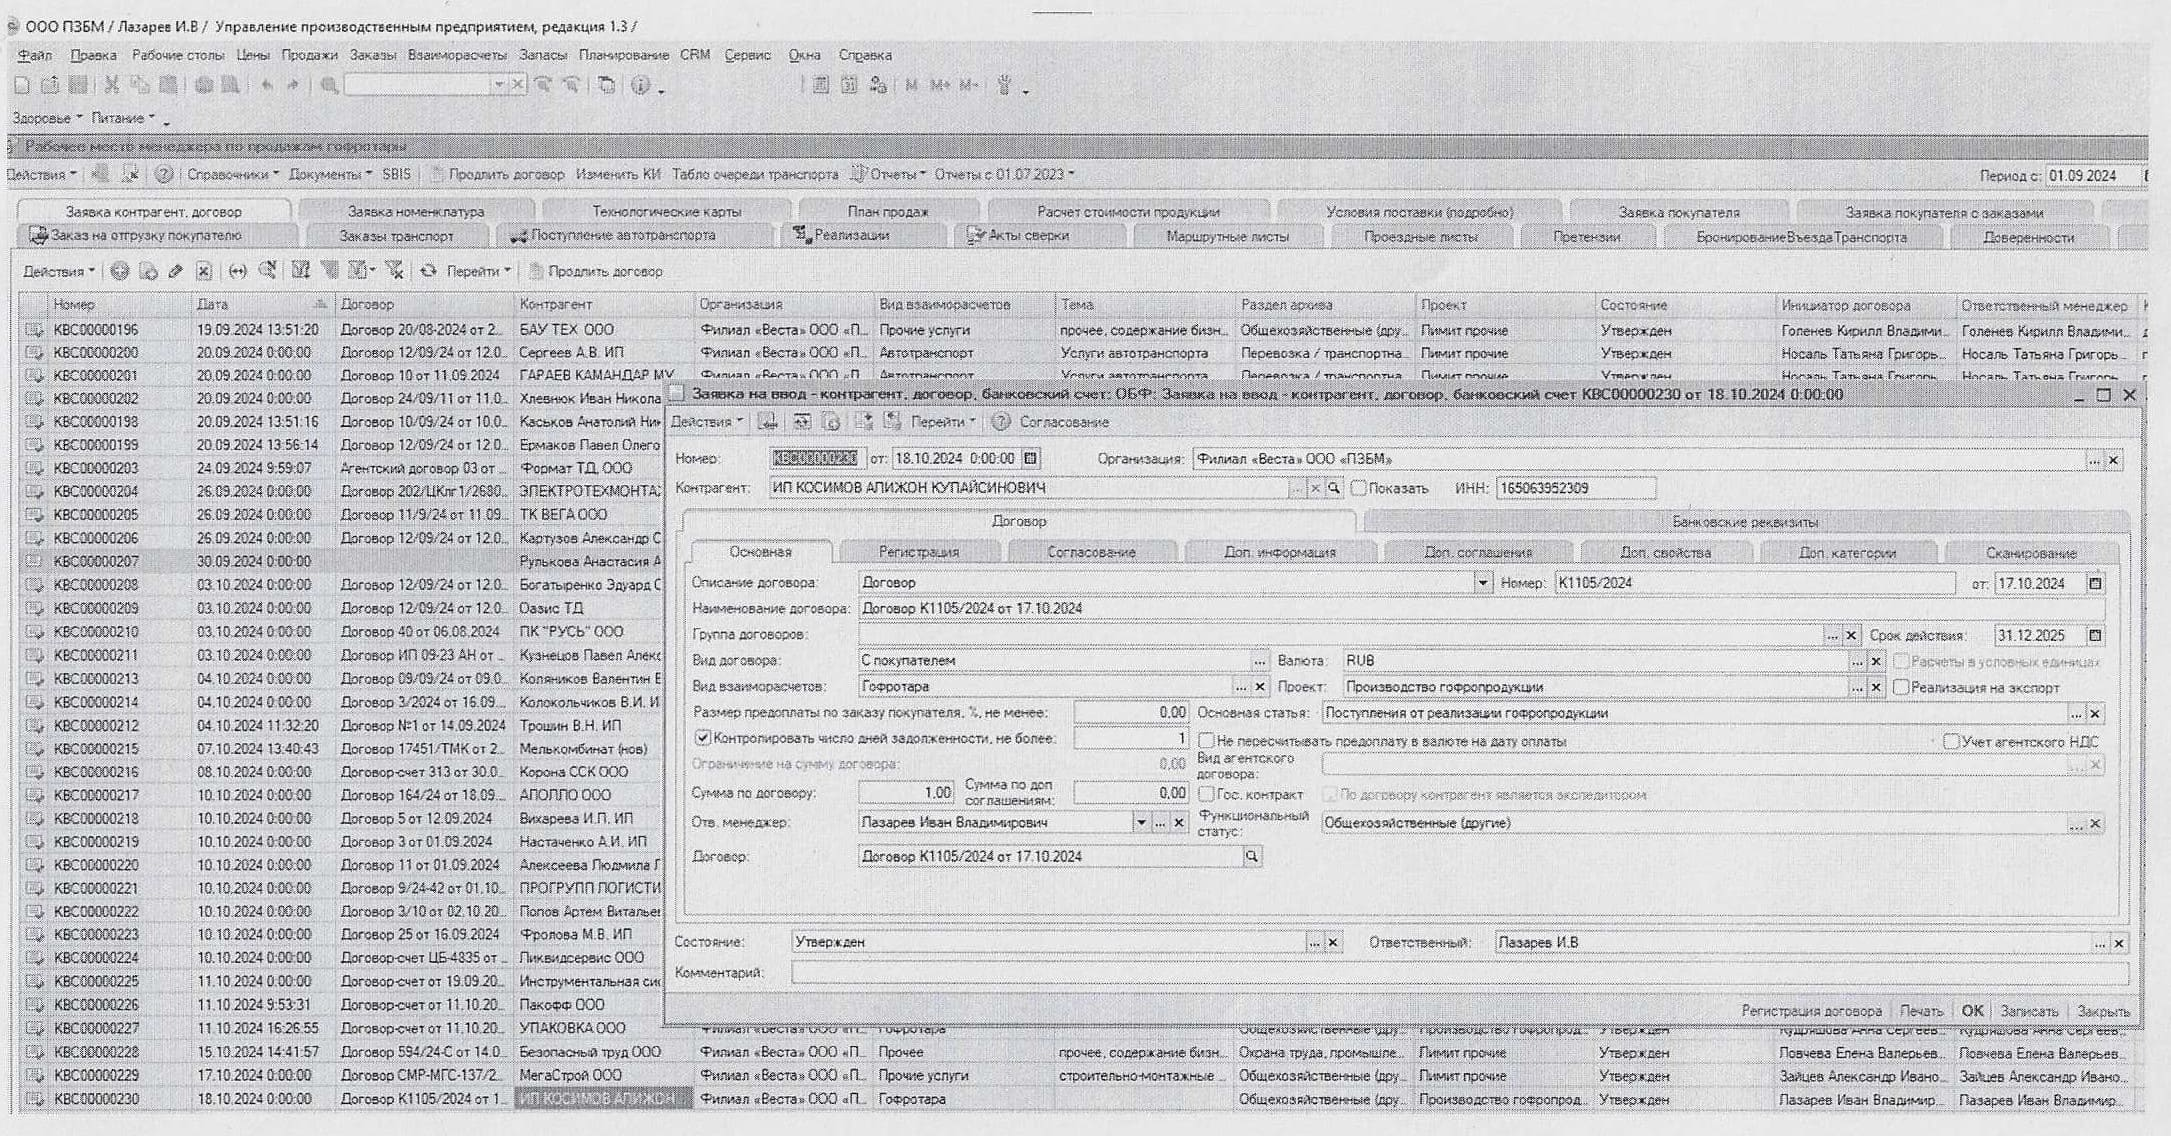
\includegraphics[height=0.35\textheight, width=1.5\textwidth, angle=90, keepaspectratio]{Pics/I.5.2.jpg}
\end{center}
\caption{Форма заявки на ввод нового контрагента в 1С: УПП}
\label{pic:I.5.2.jpg}
\end{figure}
\clearpage

% Для расчета цены менеджер использует шаблон в MS Excel (рис. \ref{pic:pic_d2}). 
% К цене сырья добавляется стоимость на сложную высечку.  Стоимость упаковки включена в цену изделия. Таким образом менеджер определяет базовую нормативную себестоимость продукции.  Цена продажи определяется менеджером исходя из себестоимости и рентабельности производства.


% Каждый менеджер ведет расчет по новым изделиям в своих файлах. Менеджер заносит в файл наименование изделия (обычно контрагент) длину, ширину, высоту (внутренние размеры изделия). По формуле будет рассчитана площадь изделия. Менеджер выбирает сырье по композиции. 
% Менеджер подбирает сырье по аналогии либо по истории такой же коробки. 

% При необходимости изготовления сложной высечки менеджер  запрашивает у контрагента чертеж или образец (процесс ''Изготовление образцов продукции'' \ref{bp:pattern}).

% На основании расчета (рис. \ref{pic:pic_d2}) менеджер формирует коммерческое предложение (рис. \ref{pic:pic_d3}). Для печати предложения используется шаблон.
% На основе полученного результата расчета себестоимости изделия менеджер  формирует коммерческое предложение и высылает его заказчику (рис. \ref{pic:pic_d3}). Для печати предложения используется шаблон. Номер КП указывается по порядку. В коммерческом предложении указывается наименование гофропродукции, марка, профиль и цена изделия. Цена актуальна в течение месяца. 
% Коммерческое предложение высылается заказчику для согласования.
% Все предложения менеджер фиксирует в таблице MS Excel предложения  (рис. \ref{pic:pic_d4}).


% Менеджер высылает КП заказчику.
% Заказчик высылает менеджеру согласованное предложение с реквизитами для заключения договора. Менеджер формирует договор поставки и высылает заказчику на согласование. В дополнение к договору менеджер формирует спецификацию на цену продукции, где указывается согласованный перечень поставляемой продукции и цены на нее (рис. \ref{pic:pic_d5}). Дополнительное соглашение является дополнением к договору. Все документы заполняются менеджером вручную.
% После согласования заказчиком коммерческого предложения менеджер запрашивает карточку контрагента для заключения договора. Менеджер отправляет в офис Московский карточку контрагента и спецификацию (рис. \ref{pic:pic_d5}) для заключения договора.

% Секретарь формирует договор с заказчиком, присваивает номер дату и высылает договор менеджеру по электронной почте. Менеджер согласует договор с заказчиком. Заказчик подписывает договор. Менеджер передает в бухгалтерию карточку заказчика и копию подписанного договора. 
% Отдел учета в системе 1С Предприятие 7.7 Бухгалтерия  создаёт  справочнике ''Контрагенты'' нового заказчика и договор.

% После выставления счета менеджер контролирует оплату от заказчика. Контроль оплаты менеджер выполняет в программе 1С 7.7. Бухгалтерия. В системе 1С 8.3 ''Бухгалтерия предприятия'' ведётся  учет поступления денежных средств на расчётный счёт, но с опозданием.
% Банк ведется в двух системах: 1С 7.7. Бухгалтерия и 1С 8.3 ''Бухгалтерия предприятия''.


%Менеджер получает запрос только по почте менеджер создает заявку на расчёт \ref{pic:calculation1}.
%Менеджер звонит на производство специалисту по планированию, который присваивает номер гофроизделия в файле ''Начало''.
%Менеджер подбирает сырье для производства изделия самостоятельно, при это есть таблица компоновок сырья \ref{pic:Layerscost}, которая не используется. Менеджер определяет количество на поддоне. При указании вида транспорта менеджер рассчитывает стоимость доставки \ref{pic:transportcost}. Менеджер рассчитывает количество поддонов, чтобы посчитать затраты на доставку. Особые условия указанной в условиях упаковке.
%
%Файл  \ref{pic:calculation1} отправляется экономисту почтой. 
%
% Расчет предварительной стоимости изделия выполняет МАП в системе 1С:УНФ при получении заявки от покупателя. Цена для продажи рассчитывается исходя из суммы следующих слагаемых.
% \begin{itemize}
% \item Стоимость гофрокартона -- рассчитывается как стоимость одного метра гофрокартона определенного профиля.
% \item Наценка за печать -- менеджер указывает примерную площадь запечатки краской в процентах. Процент запечатки учитывается при расчете затрат на печать.
% \item Паллетирование -- если для изделия требуется укладка на поддон, то стоимость паллетирования добавляется в стоимость изделий. Стоимость паллетирования одного изделия рассчитывается как стоимость паллетирования одного поддона, деленная на количество изделий на поддоне.
% \item Затраты на упаковку;
% \item Транспортировка -- стоимость доставки готовой продукции до получателя на единицу продукции.
% \end{itemize}
%
%
% \begin{figure}
% \begin{center}
%   \includegraphics[width=\linewidth, height=0.94\textheight, keepaspectratio]{Pics/d1.jpg}
% \end{center}
%   \caption{Форма расчета стоимости нового изделия}
%   \label{pic:d1}
% \end{figure}
% \clearpage
%
%
% \begin{figure}
% \begin{center}
%   \includegraphics[width=\linewidth, height=0.94\textheight, keepaspectratio]{Pics/d5.jpg}
% \end{center}
%   \caption{Форма коммерческого предложения}
%   \label{pic:d5}
% \end{figure}
% \clearpage

%
%%
% \begin{figure}
% \begin{center}
%   \includegraphics[width=\linewidth, height=0.94\textheight, keepaspectratio]{Pics/d5.jpg}
% \end{center}
%   \caption{Форма коммерческого предложения}
%   \label{pic:d3}
% \end{figure}
% \clearpage


% \begin{figure}
% \begin{center}
%   \includegraphics[width=\linewidth, height=0.94\textheight, keepaspectratio]{Pics/d6.jpg}
% \end{center}
%   \caption{Форма спецификации к договору}
%   \label{pic:d6}
% \end{figure}
% \clearpage

% \begin{figure}
% \begin{center}
%   \includegraphics[width=\linewidth, height=0.94\textheight, keepaspectratio]{Pics/pic_d5.jpg}
% \end{center}
%   \caption{Форма спецификации к договору}
%   \label{pic:pic_d5}
% \end{figure}
% \clearpage

%
%\begin{figure}
%\begin{center}
%\ifnum\pdfoutput=0
%  \includegraphics[40,0][366,292]{Pics/03_calculation2.png}
%\else 
%  \includegraphics[width=\linewidth, height=0.94\textheight, keepaspectratio]{Pics/03_calculation2.jpg}
%\fi
%\end{center}
%  \caption{Расчет стоимости изделия от экономиста.}
%  \label{pic:calculation2}
%\end{figure}
%\clearpage
%
%
%\begin{figure}
%\begin{center}
%\ifnum\pdfoutput=0
%  \includegraphics[40,0][366,292]{Pics/03_calculation3.png}
%\else 
%  \includegraphics[width=\linewidth, height=0.94\textheight, keepaspectratio]{Pics/03_calculation3.jpg}
%\fi
%\end{center}
%  \caption{Упрощенный расчет стоимости.}
%  \label{pic:calculation3}
%\end{figure}
%\clearpage
%
%
%

%
%
%\begin{figure}
%\begin{center}
%\ifnum\pdfoutput=0
%  \includegraphics[40,0][366,292]{Pics/04_KP1.png}
%\else 
%  \includegraphics[width=\linewidth, height=0.94\textheight, keepaspectratio]{Pics/04_KP1.jpg}
%\fi
%\end{center}
%  \caption{Коммерческое предложение.}
%  \label{pic:KP1}
%\end{figure}
%\clearpage
%
%
%\begin{figure}
%\begin{center}
%\ifnum\pdfoutput=0
%  \includegraphics[40,0][366,292]{Pics/34_contract.png}
%\else 
%  \includegraphics[width=\linewidth, height=0.94\textheight, keepaspectratio]{Pics/34_contract.jpg}
%\fi
%\end{center}
%  \caption{Договор поставки.}
%  \label{pic:contract}
%\end{figure}
%\clearpage
%
%
%\begin{figure}
%\begin{center}
%\ifnum\pdfoutput=0
%  \includegraphics[40,0][366,292]{Pics/07_specification_for_contract.png}
%\else 
%  \includegraphics[width=\linewidth, height=0.94\textheight, keepaspectratio]{Pics/07_specification_for_contract.jpg}
%\fi
%\end{center}
%  \caption{Спецификация к договору поставки.}
%  \label{pic:specificationforcontract}
%\end{figure}
%\clearpage
%
%
%
%
%
%
%
%
%
%
%%Расчет предварительной стоимости изделия выполняется в отделе маркетинга при получении заявки от покупателя.
%%
%%Технолог ОМ заполняет таблицу по расчету предварительной себестоимости изделия (см. рис.\ref{pic:Calculation}. Экономист в структуре ОМ выполняет по данному расчету расчет себестоимости изделия для покупателя. Для расчета используются нормативные цены для расчета стоимости изделия (рис. \ref{pic:Compound},  \ref{pic:CompoundPrint}, \ref{pic:CalculationPack}, \ref{pic:CompoundPrint}).
%%
%%На основе полученного результата расчета себестоимости изделия менеджер ОМ формирует коммерческое предложение и высылает заказчику. Согласованное заказчиком предложение с реквизитами для заключения договора покупатель высылает в ОМ. Менеджер передает заявку юристу для составления и согласования договора. Экономист в структуре ОМ формирует спецификацию к договору. В спецификации указывается условия производства, отгрузки и поставки продукции (рис. \ref{pic:Offer}).
%%
%%На основании согласованной с заказчиком и подписанной заявки технологи ОМ разрабатывают технологическую карту изделия (см. процесс ''Подготовка производства'' \ref{bp:Prepare}).
%
%%\begin{figure}
%%\begin{center}
%%  \includegraphics[height=0.94\textheight, keepaspectratio]{Pics/Calculation.jpg}
%%\end{center}
%%  \caption{Форма заполнения расчета для нового изделия}
%%  \label{pic:Calculation}
%%\end{figure}

% \clearpage
% \begin{figure}
% \begin{center}
%  \includegraphics[height=0.7\textheight, keepaspectratio]{Pics/dd5.jpg}
% \end{center}
%  \caption{Карточка организации в СБИС}
%  \label{pic:dd5}
% \end{figure}


% \begin{figure}
% \begin{center}
%  \includegraphics[height=0.5\textheight, keepaspectratio]{Pics/dd3.jpg}
% \end{center}
%  \caption{Форма расчета цены готовой продукции}
%  \label{pic:dd3}
% \end{figure}

% \begin{figure}
% \begin{center}
%  \includegraphics[height=0.94\textheight, keepaspectratio]{Pics/dd4.jpg}
% \end{center}
%  \caption{Форма коммерческого предложения}
%  \label{pic:dd4}
% \end{figure}
% \begin{figure}
% \begin{center}
%  \includegraphics[height=0.3\textheight, keepaspectratio]{Pics/dd6_1.jpg}
% \end{center}
%  \caption{Форма карточки номенклатуры готовой продукции}
%  \label{pic:dd6_1}
% \end{figure}


% \begin{figure}
% \begin{center}
%  \includegraphics[height=0.4\textheight, keepaspectratio]{Pics/dd8.jpg}
% \end{center}
%  \caption{Форма счета}
%  \label{pic:dd8}
% \end{figure}


% %
% \clearpage
% \ifx \notincludehead\undefined
\normalsize
\end{document}
\fi